\documentclass{beamer}

% Setup appearance:

\usetheme{Darmstadt}
\usecolortheme{albatross}
%\usetheme{Copenhagen}
%\usetheme{AnnArbor}
\usefonttheme[onlylarge]{structurebold}
\setbeamerfont*{frametitle}{size=\normalsize,series=\bfseries}
\setbeamertemplate{navigation symbols}{}

\definecolor{MWBlood}{rgb}{0.278, 0.0, 0.016} % MWBlood (primary)
\definecolor{MWBloodDark}{rgb}{0.039, 0.0, 0.0} % MWBloodDark (secondary)
\definecolor{MWBloodMiddle}{rgb}{0.171, 0.00, 0.01} % MWBloodMiddle ()
\definecolor{MWBone}{rgb}{0.827, 0.827, 0.827} % MWBone (Text)

\setbeamercolor{palette primary}{bg=MWBlood,fg=MWBone} % Slide heading and title box background.
\setbeamercolor{palette secondary}{bg=MWBloodMiddle, fg=MWBone}
\setbeamercolor{palette tertiary}{bg=green,fg=MWBone}
\setbeamercolor{palette quaternary}{bg=MWBloodDark, fg=MWBone} % Navigation bar
\setbeamercolor{background canvas}{bg=MWBloodDark, fg=green}
\setbeamercolor{normal text}{fg=MWBone}

\setbeamercolor{sidebar}{use=structure,bg=green}
  
\setbeamercolor{palette sidebar primary}{use=structure,fg=green}
\setbeamercolor{palette sidebar secondary}{fg=green}
\setbeamercolor{palette sidebar tertiary}{use=structure,fg=green}
\setbeamercolor{palette sidebar quaternary}{fg=green}


% Standard packages

\usepackage[english]{babel}
\usepackage[utf8]{inputenc}
\usepackage{times}
\usepackage[T1]{fontenc}
\usepackage{url}
\usepackage{lettrine}

% Setup TikZ

\usepackage{tikz}
\usetikzlibrary{arrows}
\tikzstyle{block}=[draw opacity=0.7,line width=1.4cm]


% Author, Title, etc.

\title[Titel]
{
  \texttt{\huge{meta metal mapper}}\\\vspace{3 mm}
  \textit{A data science journey for software developers}
}

\author[Martin Woelke]
{
  Martin~Woelke
}

\date{Lübeck - \today}

% The main document

\begin{document}

\begin{frame}
  \titlepage
\end{frame}

\begin{frame}{Summary}
  \tableofcontents
\end{frame}


\section{Introduction}

%\pgfimage[width=.45\textwidth,page=2]{beamer}

  \subsection{meta metal mapper}

    \begin{frame}{Inspiration}
    \end{frame}

    \begin{frame}{What is metal?}
%      \uncover<1->
      \begin{center}
        \includegraphics[scale=.18]{family_tree}
      \end{center}
    \end{frame}

  \section{Statistics}

    \begin{frame}{Tools Used}
      \begin{itemize}
        \item<1-> Programming language: Python 2 and 3 on Window and Linux,
        \item<1-> IDEs: Visual Studio and PyCharm,
        \item<1-> Graphviz
        \item<1-> Markdown
        \item<1-> Neo4j (graph database)
        \item<1-> Graphviz (diagram rendering)
        \item<1-> SCM: git
        \item<1-> Gephi (graph rendering and querying)
        \item<1-> \LaTeX{}
        \item<1-> Markdown
      \end{itemize}
    \end{frame}

    \begin{frame}{History}

      \begin{itemize}

        \item<1-> First commit : 2014-03-15
        \item<1-> Some progress made till July.
          \begin{center}
            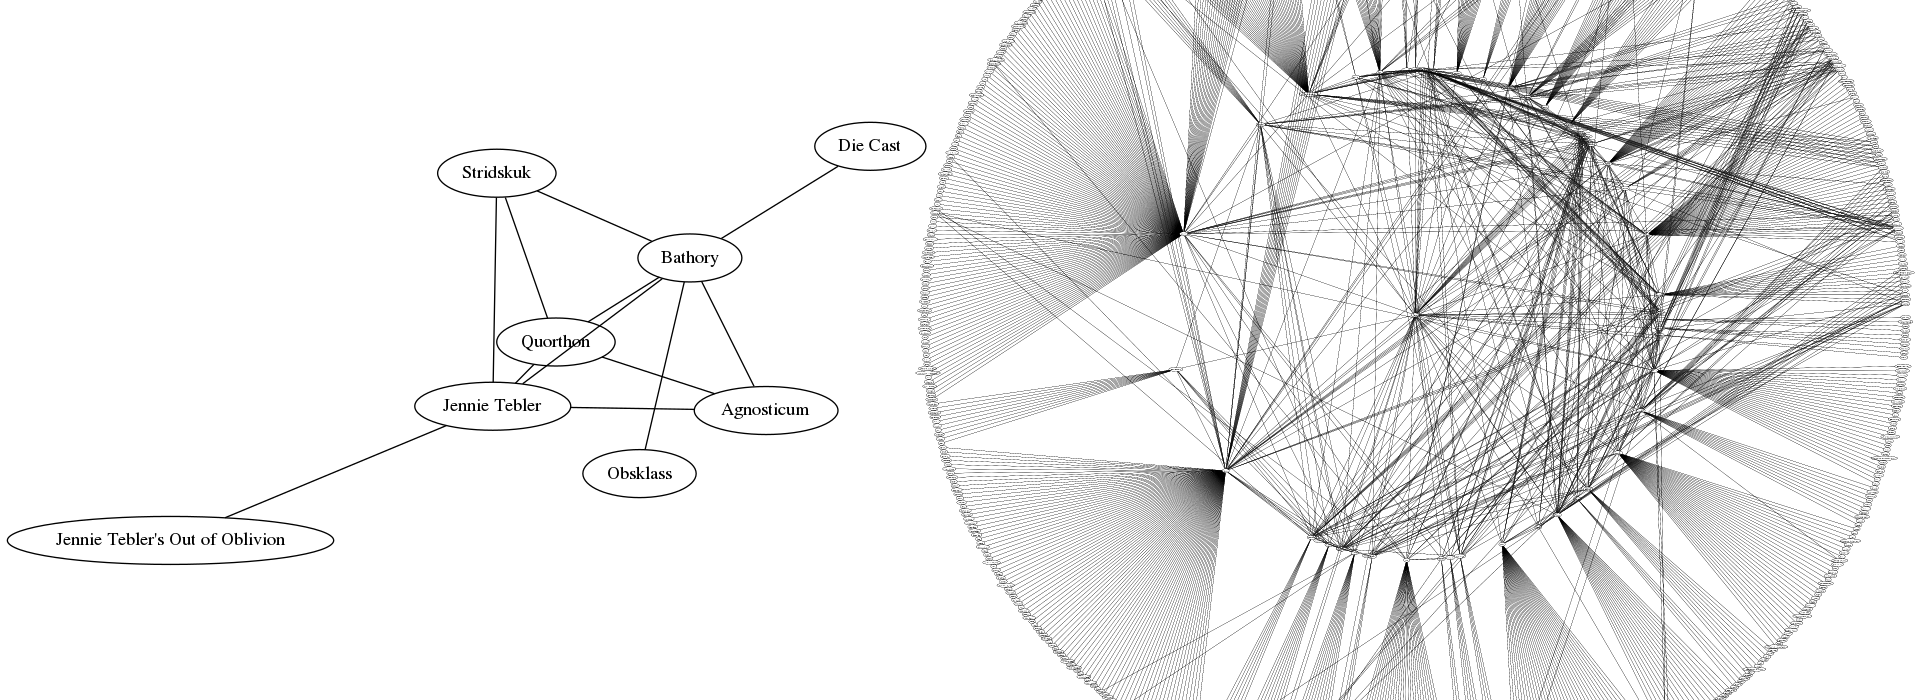
\includegraphics[scale=.6]{bandsGraphCombined}
          \end{center}
        \item<2-> Mothballed until end of 2018.
        \item<2-> 600 Commits later: ~2400 loc + 400 comments + 4k words in
          markdown.
      \end{itemize}

    \end{frame}


%%%%%%%%%%%%%%%%%%%%%%%%%%%%%%%%%%%%%%%%%%%%%%%%%%%%%%%%%%%%%%%%%%%%%%%%%
%%%%%%%%%%%%%%%%%%%%%%%%%%%%%%%%%%%%%%%%%%%%%%%%%%%%%%%%%%%%%%%%%%%%%%%%%

\section{Reporting}

  \subsection{Country Statistics}

    \begin{frame}{Most Common Styles}
      Table?
    \end{frame}


\end{document}

    \begin{frame}{}

    \end{frame}


